\documentclass[]{article}
\usepackage[utf8]{inputenc}
\usepackage[T1]{fontenc}
\usepackage{xcolor}
\usepackage{listings}
\usepackage{indentfirst}
\usepackage{hyperref}
\usepackage{graphicx}
\graphicspath{ {./wykresy/} }
\usepackage{geometry}
\usepackage{multirow}
\usepackage{color, colortbl}
\usepackage[font=small,labelfont=bf]{caption}
\usepackage{gauss} 
\usepackage{courier}

\geometry{
	a4paper,
	total={170mm,257mm},
	left=20mm,
	top=20mm,
}
\hypersetup{
	colorlinks=true,
	linkcolor=blue,
	filecolor=magenta,      
	urlcolor=cyan,
}

%opening
\title{Obliczenia naukowe. Lista nr 5. Sprawozdanie.}
\author{Kacper Szatan, nr 236478}
\date{January 6, 2020}
\begin{document}
\maketitle

\section{Opis problemu}
Przedmiotem badania jest poszukiwanie sposobu na rozwiązania układu równań liniowych postaci: $\mathbf{Ax} = \mathbf{b}$. Macierz $\mathbf{A}\epsilon \mathcal{R}^{n \times n}$, a wektor prawych storn $\mathbf{b} \epsilon \mathcal{R}^n$, dla $n \geq 4 $. Macierz $\mathbf{A}$ jest rzadka i blokowa o następującej strukturze: 
\[ \mathbf{A} = 
\begin{gmatrix}[p]
A_1 & C_1 & 0 & 0 &	0 & \ldots & 0 \\
B_2 & A_2 & C_2 & 0 & 0 & \ldots & 0\\
0 & B_3 & A_3 & C_3 & 0 & \ldots & 0\\
\vdots & \ddots & \ddots & \ddots & \ddots & \ddots & \vdots \\
0 & \ldots & 0 & B_{v-2} & A_{v-2} & C_{v-2} & 0 \\
0 & \ldots & 0 & 0 & B_{v-1} & A_{v-1} & C_{v-1} \\
0 & \ldots & 0 & 0 & 0 & B_v & A_v\\
\end{gmatrix}
\]

$v = n/l$, zakładając, że $n$ jest podzielne przez przez $l$, gdzie $l \geq 2$ oraz jest rozmiarem wszystkich wewnętrznych macierzy kwadratowych blokowych $\mathbf{B}_k, \: \mathbf{A}_k, \: \mathbf{C}_k, \: \mathbf{0}_k$. To znaczy, ze  $\mathbf{B}_k \epsilon \mathcal{R}^{l \times l}, \: \mathbf{A}_k \epsilon \mathcal{R}^{l \times l}, \: \mathbf{C}_k \epsilon \mathcal{R}^{l \times l}$ oraz macierz $ 0 \epsilon \mathcal{R}^{l \times l}$. Macierze $\mathbf{0_k}$ są wypełnione samymi zerami. Macierze $\mathbf{A_k}$ jest gęsta. W macierzach typu $\mathbf{B_k}$ wypełnione są jedynie ostatnie dwie kolumny. Natomiast macierze $\mathbf{C_k}$ są macierzami diagonalnymi, to znaczy, że mają elementy jedynie na przekątnej łączącą lewy górny róg z prawym dolnym.

Ponieważ $n$ jest bardzo duże wyklucza to użycie algorytmów bibliotecznych do rozwiązania zadango problemu. Należy wykorzystać regularność występowania elementów w macierzy oraz to, że macierz $\mathbf{A}$ jest macierzą rzadką. Co przy założeniach, że $l$ jest stałą pozwala skrócić czas obliczeń z $O(n^3)$ do $O(n)$. Zaproponowano następującę podejścia do problemu:
\begin{itemize}
	\item[1.] Zastosowanie eliminacji Gaussa, z uwzględnieniem specyficznego układu macierzy $\mathbf{A}$.
	\subitem(a) Wersja bez wyboru elementu głównego.
	\subitem(b) Wersja z częściowym wyborem elementu głównego.
	\item[2.] Zastosowanie rozkładu $\mathbf{LU}$, wyliczanego metodą eliminacji Gaussa, z uwzględnieniem specyficznego układu macierzy $\mathbf{A}$. 
	\subitem(a) Wersja bez wyboru elementu głównego.
	\subitem(b) Wersja z częściowym wyborem elementu głównego.
	\item[3.] Wyliczenie rozwiązania z wykorzystaniem wczesniej obliczonego rozkładu $\mathbf{LU}$ dla obu przypadków.
\end{itemize}
\subsection{Uwaga techniczna}
Macierz $\mathbf{A}$ jest macierzą rzadką. Zatem przechowywanie jej elementów w zwykłej tablicy dwuwymiarowej byłoby nieefektywne oraz prowadziło by do nadmiernego zużycia pamięci, która w żaden sposób nie jest wykorzystywana. Aby obejść ten problem posłużono się specjalną strukturą danych \texttt{SparseMatrixCSC} dostarczoną przez roszerzenie \texttt{SparseArrays} należące do standardu języka \texttt{julia}. Użycie tej struktury pozwala na przechowywanie w pamięci jedynie nie zerowych elementów macierzy. Na potrzeby tego laboratrium przyjmiemy, że dostęp do elementu takiej struktury jest stały.    
\section{Eliminacja Gaussa}
\subsection{Macierze łatwo obliczalne}
Wiemy, że istnieją postacie macierzy $\mathbf{A}$, które w zagadnieniu poszukiwania rozwiązania $\mathbf{Ax} = \mathbf{b}$, są łatwo obliczalne. Takimi macierzami są na przykład macierze z jednymi niezerowym elementem na przekątnej. Innym przykładem takich macierzy są macierze trójkątne, górna (\textbf{U}) i  dolna (\textbf{L}). Opiszemy teraz algorytm rozwiązujący zadany problem w przypadku gdy macierz $\mathbf{A}$ jest macierzą trójkątną górną. 

\[ 
\begin{gmatrix}[p]
a_{1,1} & a_{1,2} & \ldots & a_{1,n} \\
0 & a_{2,2} & \ldots & a_{2,n} \\
\vdots & \ddots & \ddots& \vdots \\
0 & \ldots & 0 & a_{n_n} \\
\end{gmatrix}
\begin{gmatrix}[p]
x_1 \\
x_2 \\
\vdots \\
x_n \\
\end{gmatrix}
=
\begin{gmatrix}[p]
b_1 \\
b_2 \\
\vdots \\
b_n \\
\end{gmatrix}
\]
Aby rozwiązać tak zadany układ równań załużmy, że $a_{i,i} \not = 0$. Zacznijmy analizę macierzy od ostatniego wiersza. Od razu możemy zauważyć, że $x_n = b_n/a_{n,n}$. Przechodzimy wtedy do analizy wiersza wyżej. Możemy wtedy obliczyć $x_{n-1} = \frac{b_{n-1} - x_n*a_{n-1, n} }{a_{n-1,n-1}}$ ponieważ $x_n$ mamy już obliczone z poprzedniego kroku. Po nabyciu intuicji możemy sformułować wzory rekurencyjne na obliczenie $x_i$. 
\[ x_n = b_n/a_{n,n} \]
\[ x_i =  \frac{b_{i} - \sum_{j = i+1}^{n} x_j * a_{i, j} }{a_{i,i}}\]
 Algorytm analizuje tak kolejne wiersze korzystając z wcześniej obliczonych wartości $x_i$. Po pełnym przejściu otrzymamy rozwiązanie w postaci wektora $\mathbf{x}$. Ten algorytm nazywamy algorytmem \textit{podstawiania wstecz}. Istnieje również bliźniaczy algorytm dla macieży trójątnej dolnej, w którym zaczynamy analizę nie od ostatniego, a od pierwszego wiersza i posuwamy się w dół macierzy a nie w górę. Ten algorytm nazywamy \textit{podstawianiem w przód}. Dla macierzy gęstych złożonośc tych algorytmów wynosi $O(n^2)$ ponieważ mamy jedną pętlę ,która iteruje nam po kolejnych wierszach (których jest $n$), a wewnątrz niej  obraca się petla iterująca po kolejnych kolumnach w rozpatrywanym wierszu. Wewnętrzna pętla średnio obraca się $n/2$ razy. Stąd mamy $n * n/2 = O(n^2)$. Podczas implementacji tych algorytmów do macierzy rzadkich mocno ograniczmy wewnętrzną pętlę. W najgorszym przypdaku przez $3*l$ co przy założeniu, że $l = const$ pozwala nam osiągnąć złożonośc liniową tego algorytmu.  

\subsection{Rozkład macierzy}
Podstawowy algorytm eliminacji Gaussa polega właśnie na sprowadzeniu macierzy $\mathbf{A}$ do macierzy górnej trójkątnej, a nastepnie skorzystaniu z algorytmu \textit{podstawiania wstecz}. Jest to osiągnięte za pomocą podstawowych operacji macierzowych takich jak mnożenie wiersza macierzy przez skalar oraz odejmowanie wierszów macierzy od siebie. Eliminacja Gaussa rozpoczyna działanie od góry macierzy $\mathbf{A}$ i wybiera element leżący na przekątnej. Nazwijmy go elementem głównym. Następnie element główny jest wkorzystany do wyzerowania wszystkich wyrazów należących do tej samej kolumny co element główny i znajdujących się poniżej elementu głównego. To znaczy, że element $a{i,i}$ posłuży do wyzerowania wyrazów od $a{i+1,i}$ do $a{n,i}$. Zerowanie odbywa się przez odejmowanie od siebie odpowiednich iloczynów $i-tego$ wiersza od kolejnych niżej znajdujących się wierszy. Mnożnik $i-tego$ wiersza potrzebny do wyzerowania elementu w $j-tym$ wierszu oblicza się następująco:
\[m = \frac{a_{j,i}}{a_{i,i}}\]
Następnie odejmujemy cały $i-ty$ wiersz, w którym każdy element jest pomnożony przez mnożnik od wiersza $j-tego$. Musimy jeszcze wyrównać wektor $\mathbf{B}$ do aktualnej wersji macierzy $\mathbf{A}$. Realizujemy to za pomocą tego samego mnożnika i analogicznej operacji. $(new)b_j = (old)b_j - m * b_i$. Po przeprowadzeniu tych operacji na wszytskich wierszach macierzy otrzymujemy postać górną trójkątną. Co pozwala nam wykorzystać wcześniej omówiony algorytm \textit{podstawiania wtecz}.

W algorytmie eliminacji Gaussa możemy wyróznić trzy pętle. Pierwsza iteruje po wierszach od góry jednocześnie wybierając element główny. Druga pętla przebiega wiersze, od których będziemy odejmować wiersz wyznaczony przez pętlę pierwszą. Trzecia pętla zajmuje się przebieganiem kolumn w odejmowanym wierszu w celu zaktualizowania ich wartości. W macierzy gęstej kwadratowej zewnętrzna pętla obraca się $n$ razy, a "pod" pętla druga i "pod pod" pętla trzecia średnio obrócą się $n/2$ razy. Daje to złożoność $O(n^3)$, ale podobnie jak w algorytmie \textit{podstawiania wstecz} przy założeniu, że $l = const$ udało się osiągnąć złożoność liniową.
\\\\
Zaprezentowana wyżej wersja algorytmu eliminacji Gaussa ma istotny problem, którym jest założenie, że element główny znajdujący się na diagonali macierzy \textbf{A} jest niezerowy. Rozwiązanie tego problemu przychodzi wraz z pewną modyfikacją. Mianowicie algorytmem eliminacji Gaussa z częsciowym wyborem. Modyfikacja dotyczy właśnie wyboru elementu głównego. Wiemy, że zamiana kolejności wierszy w macierzy \textbf{A} wraz z zamianą kolejnośći odpowiadającymi tym wierszom wartościami w wektorze \textbf{B} nie zmieni nam rozwiązania. Jest to czynność czysto związana z zapisem. Możemy skorzystać z tej własności, aby zabezpieczyć się przed zerowym głownym elementem. Zamiast od razu przypisywać elementowi głównemu wartości leżącą na diagonali, wyszukujemy w rozpatrywanej kolumnie wartości o największym module. Następnie wiersz w którym taka wartość się znajduje zamieniamy z aktualnie rozpatrywanym wierszem, a nowym elementem głównym staje się właśnie nasze wcześniej znalezione maksimum. W praktyce taka zamiana wierszy byłaby kosztowna dlatego stosuje się dodatkowy wektor, który zapamiętuje permutacje wierszy. Następnie ilekroć odwołujemy się do jakiegoś wiersza z macierzy \textbf{A} po prostu sprawdzamy odpowiadający mu wiersz w wektorze permutacji. Reszta algorytmu jest praktycznie taka sama jak wczesniej opisany algorytm eliminacji bez wyboru, z zachowaniem zasady o odwoływaniu się do wierszy macierzy \textbf{A} tylko za pomocą wektora permutacji. Zatem złożoność tej wersji algorytmu wciąż pozostaje $O(n^3)$, ale wyeliminowaliśmy problem z elementami zerowymi na przekątnej macierzy \textbf{A}.

\subsection{Rozkład LU}
Układu równań $\mathbf{Ax} = \mathbf{b}$, można rozwiązać z wykorzystaniem rozkładu macierzy \textbf{A} na macierze \textbf{LU}. Wtedy rozwiązanie sprowadza się do znalezienia rozwiązania następującego układu:
\[\begin{cases}
\mathbf{Lz} = \mathbf{b}\\
\mathbf{Ux} = \mathbf{z}
\end{cases}\]

Zatem jeśli chcemy otrzymać wynik, czyli interesujący nas wektor \textbf{x} to musimy rozłożyć \textbf{A} na macierze \textbf{LU}. Potem zastosować algorytm \textit{podstawiania w przód} dla pierwszego równiania z macierzą dolną trójkątną, a następnie wykorzystać wynik (wektor \textbf{z}) do policzenia równania drugiego algorytmem \textit{podstawiania wstecz}. Zatem złożoność części rozwiązującej układ równań z rozkładu \textbf{LU} to po prostu złożoność algorytu \textit{posdtawiania w przód} + \textit{podstawiania wstecz}. Co daje nam wciąż $O(n^2)$.
\\\\
Sam rozkład macierzy na macierz \textbf{L} i macierz \textbf{U} opiera się w dużej mierze na klasycznej eliminacji Gaussa. Otrzymujemy podczas niej przecież macierz \textbf{U}. Wiemy, że macierz \textbf{L} ma jedynki na przekątnej w rozkąłdzie \textbf{LU} zatem aby zaoszczędzić pamięć możemy przechowywać i macierz \textbf{L} i macierz \textbf{U} w jednej macierzy, a dokładnie w macierzy \textbf{A}. Aby wygenerować brakującą nam do obliczeń macierz \textbf{L} podczas przeprowadzania eliminacji zamiast zerować elementy pod elementem głównym zapisujemy w nich mnożnik który zostałby uzyty do wyzerowania. Tym sposobem, stosując niewielką modyfikację otrzymujemy rozkład \textbf{LU} zapisany w macierzy \textbf{A}. Oczywiście jest to realizowane w czasie $O(n^3)$ Jako, że jest to mało znacząca zmiana (jeżeli chodzi o złożoność) względem algorytmu eliminacji Gaussa.
Istnieje również wersja rozkładu \textbf{LU} z częściowym wyborem elementu głównego. Jest ona jednak analogiczna do algorytmu eliminacji Gaussa z częściowym wyborem.
\section{Zastosowane modyfikacje}
Opisane algorytmy mają niezadowalającą nas złożoność $O(n^3)$. Aby obniżyć koszty czasowe algorytmu wprowadzono szereg modyfikacji, które starają się zmniejszyć obszar rozpatrywanych wartości. Możemy to zrobić bo wiemy jak wygląda macierz \textbf{A}. We wszystkich umieszczonych wzorach $l$ długość boku macierzy wewnętrznej, a $n$ długość boku macierzy \textbf{A}.  
\subsection{Modyfikacje eliminacji Gausa bez wyboru}
Na podstawie specyficznego rozmieszczenia elementów w macierzy \textbf{A} sformułowno nastepujące wzory na ostatni niezerowy element w $i-tym$ wierszu:
\[ min(i + l, n) \]
minimum ze składnikiem $n$ ogranicza nas przez liczbę kolumn i gwarantuje nam, że nie wyjdziemy po za macierz w trakcie iteracji. W pierwszym wierszu ostatni element znajduje się właśnie na miejscu $1 + l$, a ponieważ ostatnim niezerwym elementem jest element nalerzący do macierzy wewnętrznej \textbf{C} to wiemy, że wiersz niżej ostatni element będzie jedną kolumnę dalej niż ostatni element w wierszu wyżej.
\\\\
Ostatni niezerowy element w $i-tej$ kolumnie: 
\[min(l + l * floor((i + 1)/l), n) \]
Na początku jesteśmy ograniczeni jedynie przez długość macierzy wewnętrznej \textbf{A}. Stąd pierwsze $l$ we wzorze. Następnie kiedy zaczniemy rozpatrywać kolumnę $l - 1$ ostatni wyraz nie miesci się już w wewnętrznej macierzy \textbf{A}, a w wewnętrznej macierzy \textbf{B} z wiersza niżej. Dlatego w tym momencie zwiększamy występowanie ostatniego elementu w $i-tej$ kolumnie do $2*l$. Wyrażenie $l * floor((i + 1)/l)$ zwiększa obszar przeszukiwania o długość $l$ w momencie gdy rozpatrujemy przedostatnią kolumnę wewnętrznej macierzy \textbf{A}.


Zatem poruszając się wzdłuż kolumny rozpatrujemy conajwyżej $l+2$ wierszy, w których rozpatrujemy conajwyżej $l$ wyrazów. Co pozwala na osiągnięcie złożoności $O(l^2)$. Wciąż musimy przeprowadzić te operacje dla $n$ wierszy więc złożoność tej części algorytmu wynosi $O(n * l^2)$ Przyjmujemy, że $l$ jest stałą więc otrzymujemy złożoność $O(n)$. Tak na prawdę aby rozwiązać zadanie to musimy jeszcze przeprowadzić algorytm \textit{podstawiania wstecz}. Ale korzystając ze opracowanych wzorów na ostatni wyraz w danym wierszu. Wewnętrzna pętla tego algorytmu wykonuje maksymalnie $l$ obrotów, a zewnętrzna obraca się $n$ razy. Z tego powodu złożoność algorytmu \textit{podstawiania wsztecz i w przód} jest równa $O(n)$. Zatem złożomność całej zmodyfikowanej eliminacji Gaussa jest równa $O(n)+O(n)=O(n)$.  
     
\subsection{Modyfikacje eliminacji Gaussa z wyborem elementu głównego}
Modyfikacje były właściwie analogiczne do tych zaimplementowanych w klasycznej eliminacji Gaussa. Różnica we wzorach na wyznaczenie ostatniego elementu w danej kolumnie oraz w danym wierszu, wynika z możliwości permutowania wierszy na którą pozwala metoda częściowego wyboru. Jednakże struktura elementów  w macierzy \textbf{A} jest na tyle regularna i charakterystyczna, że pozwala na permutacje wierszy tylko w ściśle określonym zakresie. To skolei pozwala na wyznaczenie wzorów na ostatni element w $i-tym$ wierszu:
\[ min(2 * l + l * floor((i + 1) / l)), n)\]
Ostatni element w $i-tej$ kolumnie:
\[min(l + l * floor((i + 1) / l_size), n)\]
Ograniczenie pętli wewnętrznych w tym algorytmie podobine jak w jego klasycznej wersji pozwala nam osiągnąc złożoność liniową.
\subsection{Modyfikacje rozkładu LU z wyborem i bez}
Modyfikacje które przeprowadzono w rozkładach \textbf{LU} są identyczne do modyfikacji przeprowadzonych w opowiadających im wersjach algorytmu Gaussa.
\subsection{Modyfikacje rozwiązywania LU z wyborem i bez}
Te algorytmy to tak na prawdę \textit{podstawianie w przód} a nastęþnie \textit{podstawianie w tył}. Modyfikacje podstawiania w tył wyglądają identycznie jak ich wersje w eliminacji Gaussa. Dla \textit{podstawiania w przód} natomiast należało opracować wzór, który zwróci w której kolumnie znajduje się peirwszy element danego wiersza (ponieważ teraz analizujemy dolną macierz trójkątną). Dla metody bez wyboru wzór wygląda tak:
	\[max(l* floor((i - 1) / l) - 1, 1)\]
, a z wyborem tak:
\[max(l * floor((permutation[i] - 1) / l) - 1, 1)\]
\subsection{Notka}
Tak na prawdę modyfikacje algorytmów pod macierze rzadkie opierają się na ograniczenie zakresu obrotu dwóch wewnętrznych pętli w algorytmie eliminacji gaussa oraz wewnetrznej petli w algorytmie \textit{podstawiania w przód} i \textit{podstawiania wstecz}. Moglibyśmy te pętle ograniczyć z góry przez $4l$ i działanie algorytmów było by poprawne oraz zachowalibyśmy złożoność liniową ponieważ $l$ jest stałą. wzory, które podano wyżej są poprostu lepszym ograniczeniem tych pętli bo bardziej dokładnym. Wynikają one wprostu z układu macierzy oraz możliwych jej permutacji po zastosowaniu algorytmu częściowego wyboru. 
\newpage
\section{Wyniki eksperymentów}
\begin{table}[h]
	\centering
	\begin{tabular}{|c c c c c c|} 
		\hline
		$n$ & $l$ & metoda & błąd względny & czas (s) & pamieć\\
		\hline\hline
		16 & 4 & Gauss & 4.871083751574258e-16 & 0.000026 & 3.750 KiB \\
		16 & 4 & Gauss z wyborem & 5.633766544994711e-16 & 0.000032 & 3.953 KiB \\
		10000 & 4 & Gauss & 3.606694893340484e-14 & 0.246179 & 1.221 MiB \\
		10000 & 4 & Gauss z wyborem & 4.631320331499356e-16 & 0.313257 & 1.297 MiB\\
		50000 & 4 & Gauss & 1.017091150895571e-13 & 7.111061 & 6.104 MiB \\
		50000 & 4 & Gauss z wyborem & 5.466808519995741e-16 &  12.448784 & 6.485 MiB \\
		\hline
	\end{tabular}
\end{table}

\begin{table}[h]
	\centering
	\begin{tabular}{|c c c c c|} 
		\hline
		$n$ & $l$ & metoda rozkładu & czas (s) & pamieć\\
		\hline\hline
		16 & 4 & LU  &  0.000017 & 3.344 KiB \\
		16 & 4 & LU z wyborem & 0.000028 & 3.547  KiB \\
		10000 & 4 & LU  & 0.246517 & 1.068 MiB \\
		10000 & 4 & LU z wyborem  & 0.254995 & 1.144 MiB\\
		50000 & 4 & LU  & 7.698057 & 5.341 MiB \\
		50000 & 4 & LU z wyborem &  10.820273 &  5.722 MiB \\
		\hline
	\end{tabular}
\end{table}

\begin{table}[h]
	\centering
	\begin{tabular}{|c c c c c c|} 
		\hline
		$n$ & $l$ & metoda rozwiązania LU & błąd względny & czas (s) & pamieć\\
		\hline\hline
		16 & 4 & LU & 4.871083751574258e-16 &  0.000006 & 992 bytes\\
		16 & 4 & LU z wyborem & 5.633766544994711e-16 & 0.000009 & 992 bytes \\
		10000 & 4 & LU & 3.606694893340484e-14 & 0.001160 & 312.969 KiB\\
		10000 & 4 & LU z wyborem & 4.631320331499356e-16 & 0.002075  & 312.969 KiB\\
		50000 & 4 & LU & 1.017091150895571e-13 & 0.003708 & 1.526 MiB \\
		50000 & 4 & LU z wyborem & 5.466808519995741e-16 &  0.009222 & 1.526 MiB \\
		\hline
	\end{tabular}
\end{table}



\begin{minipage}{0.8\linewidth}
	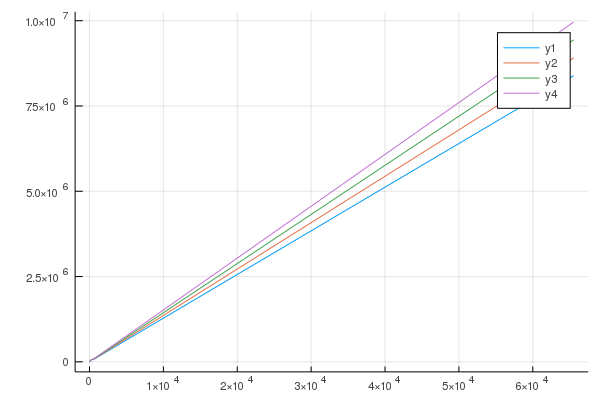
\includegraphics[width=\linewidth]{memo.png}
	\captionof{figure}{Wykres przedstawiający zużycie pamięci. $y1 = GAUSS$, $y2 = GAUSS$ z częsciowym wyborem, $y3 = GAUSS z częsciowym wyborem$, $y3 = LU$, $y4 = LU$ z częsciowym.}
\end{minipage}

\begin{minipage}{0.8\linewidth}
	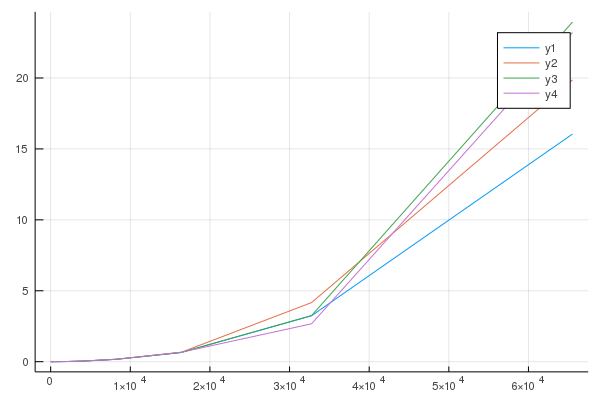
\includegraphics[width=\linewidth]{time.png}
	\captionof{figure}{Wykres przedstawiający zużycie czasowe. $y1 = GAUSS$, $y2 = GAUSS$ z częsciowym wyborem, $y3 = GAUSS z częsciowym wyborem$, $y3 = LU$, $y4 = LU$ z częsciowym. Najprawdopodobniej liniowość osiągnięta tylko na konkretnych przedziałach ma związek z założeniem, że dostęp do elementu \texttt{SparseMatrixCSC} uważamy za stały gdy tak na prawdę nie jest taki.}
\end{minipage}
\section{Wnioski} 
Metody stosujące częściowy wybór są trochę wolniejsze i zużywają więcej pamięci co zrozumiałem, ale w zamian dają nam możliwość liczenia układów równań, gdzie na diagonali maicerzy \textbf{A} są zera, zwykle dają też dokładniejsze wyniki. Możemy zauważyć, że policzenie rozwiązania z macierzy rozłożonej na \textbf{LU} trwa jedynie ułamek czasu poświęconego na samo stworzenie rozkładu. Rozkład \textbf{LU} ma przewagę nad standardowową eliminacją Gaussa, gdy chcemy testować np. jedną macierz \textbf{A} dla róznych wektorów prawych stron \textbf{B}. Bo tylko raz wyznaczymy rozkład, który kosztuje nas najwięcej przy metodzie z rozkładem \textbf{LU}. Wtedy policzenie nowego rozwiązania dla innego wektora \textbf{B} jest bardzo szybkie i zajmuje mało pamięci. Realizując zadanie udało nam się drastycznie zmniejszyć złożoność algorytmów oraz ich zapotrzebowanie pamięciowe, co pokazuje, że wiedza na temat danych z którymi się pracuje potrafi być równie ważna co znajomość algorytmów.

\end{document}